
\subsection{研究意义}
波动方程是二阶双曲型偏微分方程\cite{bedford1994},可用于描述地震波、水波、电磁波等自然界中波传播的现象,广泛的应用于无损检测、地震预测、生物医学成像等工程领域。
发展波动方程的高精度分析方法将有助于提升设计精度、降低测试成本。
由于实际工程问题中通常涉及复杂几何区域、材料非均质等一系列问题,采用理论分析手段研究工程中的波动问题难以获得解析解。因此,数值仿真分析成为了求解波动方程的重要工具。
在主流的波动方程数值分析方法中\cite{hughes2000},时间域和空间域通常独立离散为有限个分布节点用于近似位移变量,其中空间域通常采用基于变分原理的弱形式进行离散分析,如有限元法等。
弱形式型的方法具有求解精度高、稳定性强的特点,适用于复杂空间几何构型。
而时间域则采用基于微分方程的强形式进行离散分析,如有限差分法等。
强形式型方法通常采用迭代求解,过程实现简单高效。
但强形式型的方法在计算精度和稳定性方面均低于弱形式型的方法,计算误差也随着迭代步的增加而累积增大。

波动方程数值分析的另一种思路是将时间域作为第四维空间进行混合离散,时空区域均采用基于哈密顿变分原理的伽辽金弱形式进行求解,称为时空混合离散伽辽金法。
该类方法将提升整体的求解精度,有利于时空区域自适应节点加密过程。
求解过程无需进行迭代,可采用整体并行计算求解提高效率。
\textbf{
然而,时空混合离散伽辽金法在求解稳定的前提下并不能适用于任意节点分布情况,导致其未能广泛应用于复杂的实际工程问题中,阻碍了时空混合离散伽辽金法的应用和发展。
}
造成该问题的原因主要有三点:

首先是\textbf{时域末端虚位移本质边界条件的施加问题}。
波动方程的时空混合离散伽辽金法通过哈密顿变分原理建立相对应的弱形式,
如图 \ref{fg:hamilton} 所示,哈密顿原理要求虚位移$\delta q$在初始时刻$t_0$和末端时刻$t_1$为零,即$\delta q(t_0)=\delta q(t_1)=0$,以等价于欧拉--拉格朗日方程\cite{arnold1978}。
在传统边值问题中,虚位移本质边界条件通常伴随着位移本质边界条件。
采用伽辽金法进行求解时,位移及其虚位移在本质边界处的自由度数量相同。
采用矩阵压缩技术直接施加本质边界条件时,可保持刚度矩阵为方阵且可逆。
然而,波动方程在时间维度上属于初值问题,即已知初始时刻位移和速度,$q(t_0)=q_0,\dot q(t_0) = \dot q_0$,而时域末端边界条件未知。
如图 \ref{fg:direct} 所示,
采用直接施加本质边界条件时,初始时刻位移边界条件将填补末端时刻虚位移为零造成刚度矩阵却是的部分。
此时,初始时刻虚位移不再要求为零,初始时刻速度边界条件可在此处作为自然边界条件施加。
但该过程可实施的前提是\textbf{初始时刻和末端时刻的自由度数量需要保持一致,并不适用于任意节点分布情况。}

\begin{figure}[!h]
    \centering 
    \includegraphics[width=\textwidth]{figures/Hamilton.png}
    \caption{哈密顿原理与欧拉--拉格朗日方程等价性}
    \label{fg:hamilton}
\end{figure}

\begin{figure}[!h]
    \centering 
    \includegraphics[width=0.8\textwidth]{figures/stiffness.png}
    \caption{直接施加时域末端虚位移本质边界条件}
    \label{fg:direct}
\end{figure}

其次是\textbf{数值色散问题}。
数值色散问题是由于离散控制方程的局部截断误差过大,导致不同频率波的波速不一致引起的数值振荡现象\cite{zhang2024}。
抑制数值色散现象主要通过以下方法:
\textcircled{\textbf{\small 1}}
调整时间域与空间域节点离散间距,以满足Courant–-Friedrichs-–Lewy(CFL)条件或谱半径稳定性条件,提高波近似精度。
该方法需要限制节点间距比例,不适用于任意节点分布情况。
\textcircled{\textbf{\small 2}}
引入人工耗散项缓解高频振动,该方法通常需要引入微分方程作为稳定人工耗散项,微分方程中包含变量的高阶导数,不适合线性近似方案。
且人工耗散项可能会引起数值耗散问题,降低计算精度。
\textcircled{\textbf{\small 3}}
提高时域离散阶次,以降低局部截断误差,缓解振荡现象。
该方法相较于前两种方法更为直接有效,且适用于任意节点分布情况。
然而,\textbf{构造高阶形函数对于基于单元拓扑信息近似的有限元法来说并非易事,特别是对于高维时空域混合离散情况。}

最后是\textbf{高维度网格划分问题}。
相较于时间域和空间域单独离散的情况,时空混合离散需要采用高一维度的近似方案进行分析。
传统有限元法在复杂区域划分网格难度将随着维度和近似阶次的增加而提升,通常需要人工修正网格以保证计算结果的可靠性。
如图所示,传统有限元法在节点局部加密处,网格数量也随之增加。
难以保证网格质量,影响求解精度。

不同于传统有限元法,无网格法\cite{Zhang2004a}是一类仅依据节点位置信息构建高阶光滑形函数的近似方法。
在众多无网格近似方案中,再生核无网格近似可构造满足任意阶次一致性条件的无网格形函数。
\textbf{在任意节点分布下,再生核无网格近似可通过分别调整时间域和空间域的近似阶次,以降低局部截断误差,缓解数值色散引起的振荡现象。}
无网格法虽然在建立形函数过程中无需依赖网格,但在结合伽辽金法求解时,仍然需要网格作为背景积分域进行数值积分。
与有限元法不同的是,如图所示,伽辽金无网格法无需采用无网格节点作为背景积分域顶点。
采用结构型网格作为背景积分域也适用于自适应节点加密过程。
而\textbf{无网格法自适应节点加密过程中背景积分域可以不需要随节点数增加而细划,降低高维背景积分域划分难度,有效缓解网格畸变引起的精度下降}。

针对上述时空混合离散伽辽金法的瓶颈问题,本项目拟研究时空混合离散伽辽金法中虚位移本质边界条件施加方案,并结合再生核近似的伽辽金无网格法缓解数值色散问题,建立高维时空混合离散自适应节点加密方案,
旨在为波动问题发展一种适应于任意节点分布的稳定伽辽金无网格分析方法,为实际工程中的波动问题提供一种精确、鲁棒和高效的数值工具。

\subsection{国内外研究现状及发展动态}

国内外诸多学者针对时空混合离散伽辽金无网格法的相关问题进行了广泛的研究,主要研究内容可归纳为时空混合离散方案、数值色散问题稳定方案和时空混合离散无网格法三方面,下面将分别对这三方面的研究现状及发展动态进行介绍。

时空混合离散分析方法的发展可追溯到上世纪70代初\cite{argyris1969a},最早的方法直接通过哈密顿变分原理弱形式结合连续有限元近似进行构建,称为时空有限元法。
% 为规避哈密顿原理中虚位移在时域边界等于零的要求,Bailey\cite{bajer1986}直接在弱形式中消除哈密顿原理中的时域边界项(图 \ref{fg:hamilton} 中标红项),但该方法在波动方程中将存在较大的相位误差\cite{bajer1986}。
% Baruch和Riff\cite{baruch1982}对时空混合离散中,施加不同的虚位移边界条件时求解的稳定性进行探讨,证明了施加虚位移本质边界条件的重要性。
% Peters和Izadpanah\cite{peters1988}采用图 \ref{fg:direct} 所示矩阵替换法施加虚位移本质边界条件,但该方法要求初始时刻和末端时刻虚位移相关自由度数量相等。
该类方法通常采用如图 \ref{fg:direct} 所示矩阵替换法施加虚位移本质边界条件,但需要初始时刻和末端时刻虚位移相关自由度数量相等。
通过卷积理论可将哈密顿变分原理转化为Gurtin变分原理进行求解,可无需时域末端虚位移边界条件\cite{Peng1992},但卷积过程并不适用于复杂几何求解区域。
由于时间维度弱形式离散方案中虚位移在时域本质边界条件施加困难,学者们开始尝试在时域强形式离散下的时空混合离散分析方法,如强形式型的伽辽金法\cite{Li2017a}、最小二乘法\cite{epstein2024}等。
相较于时域弱形式离散,时域强形式中包含变量对时间的二阶导数,需要引入高阶近似方案进行求解。同时,时域强形式离散整体能量难以保证,求解稳定性较差。
为解决离散阶次和稳定性问题,Hughes和Hulbert\cite{hughes1988,hulbert1990}在时域强形式离散的基础上引入速度变量,将二阶偏微分方程转换为两个一阶偏微分方程,从而降低了对近似阶次的要求。
并引入时间非连续的有限元近似方案提高整体求解的稳定性,建立时空混合离散间断伽辽金法。
间断伽辽金法依据其计算精度和稳定上的优势,成为了主流的时空混合离散分析方法,诸多研究工作均以该方法为基础进行,如虚单元间断伽辽金法\cite{xu2025}、等几何间断伽辽金法\cite{lejeunes2024}、边界元间断伽辽金法\cite{hoonhout2023}等。
然而,时空混合离散间断伽辽金方案需要在时域上采用如图 \ref{fg:slab} 所示的分块离散以保证整体A--稳定性条件\cite{hughes1988},图中$\Delta t$为时间块,两时间块之间位移不连续。
\textbf{时域分块网格不仅限制了节点的布置,而且在时域块状边界处采用非连续的位移进行近似,增加了由位移自由度数量,增加了计算的复杂度和耗时。}

\begin{figure}[!h]
    \centering 
    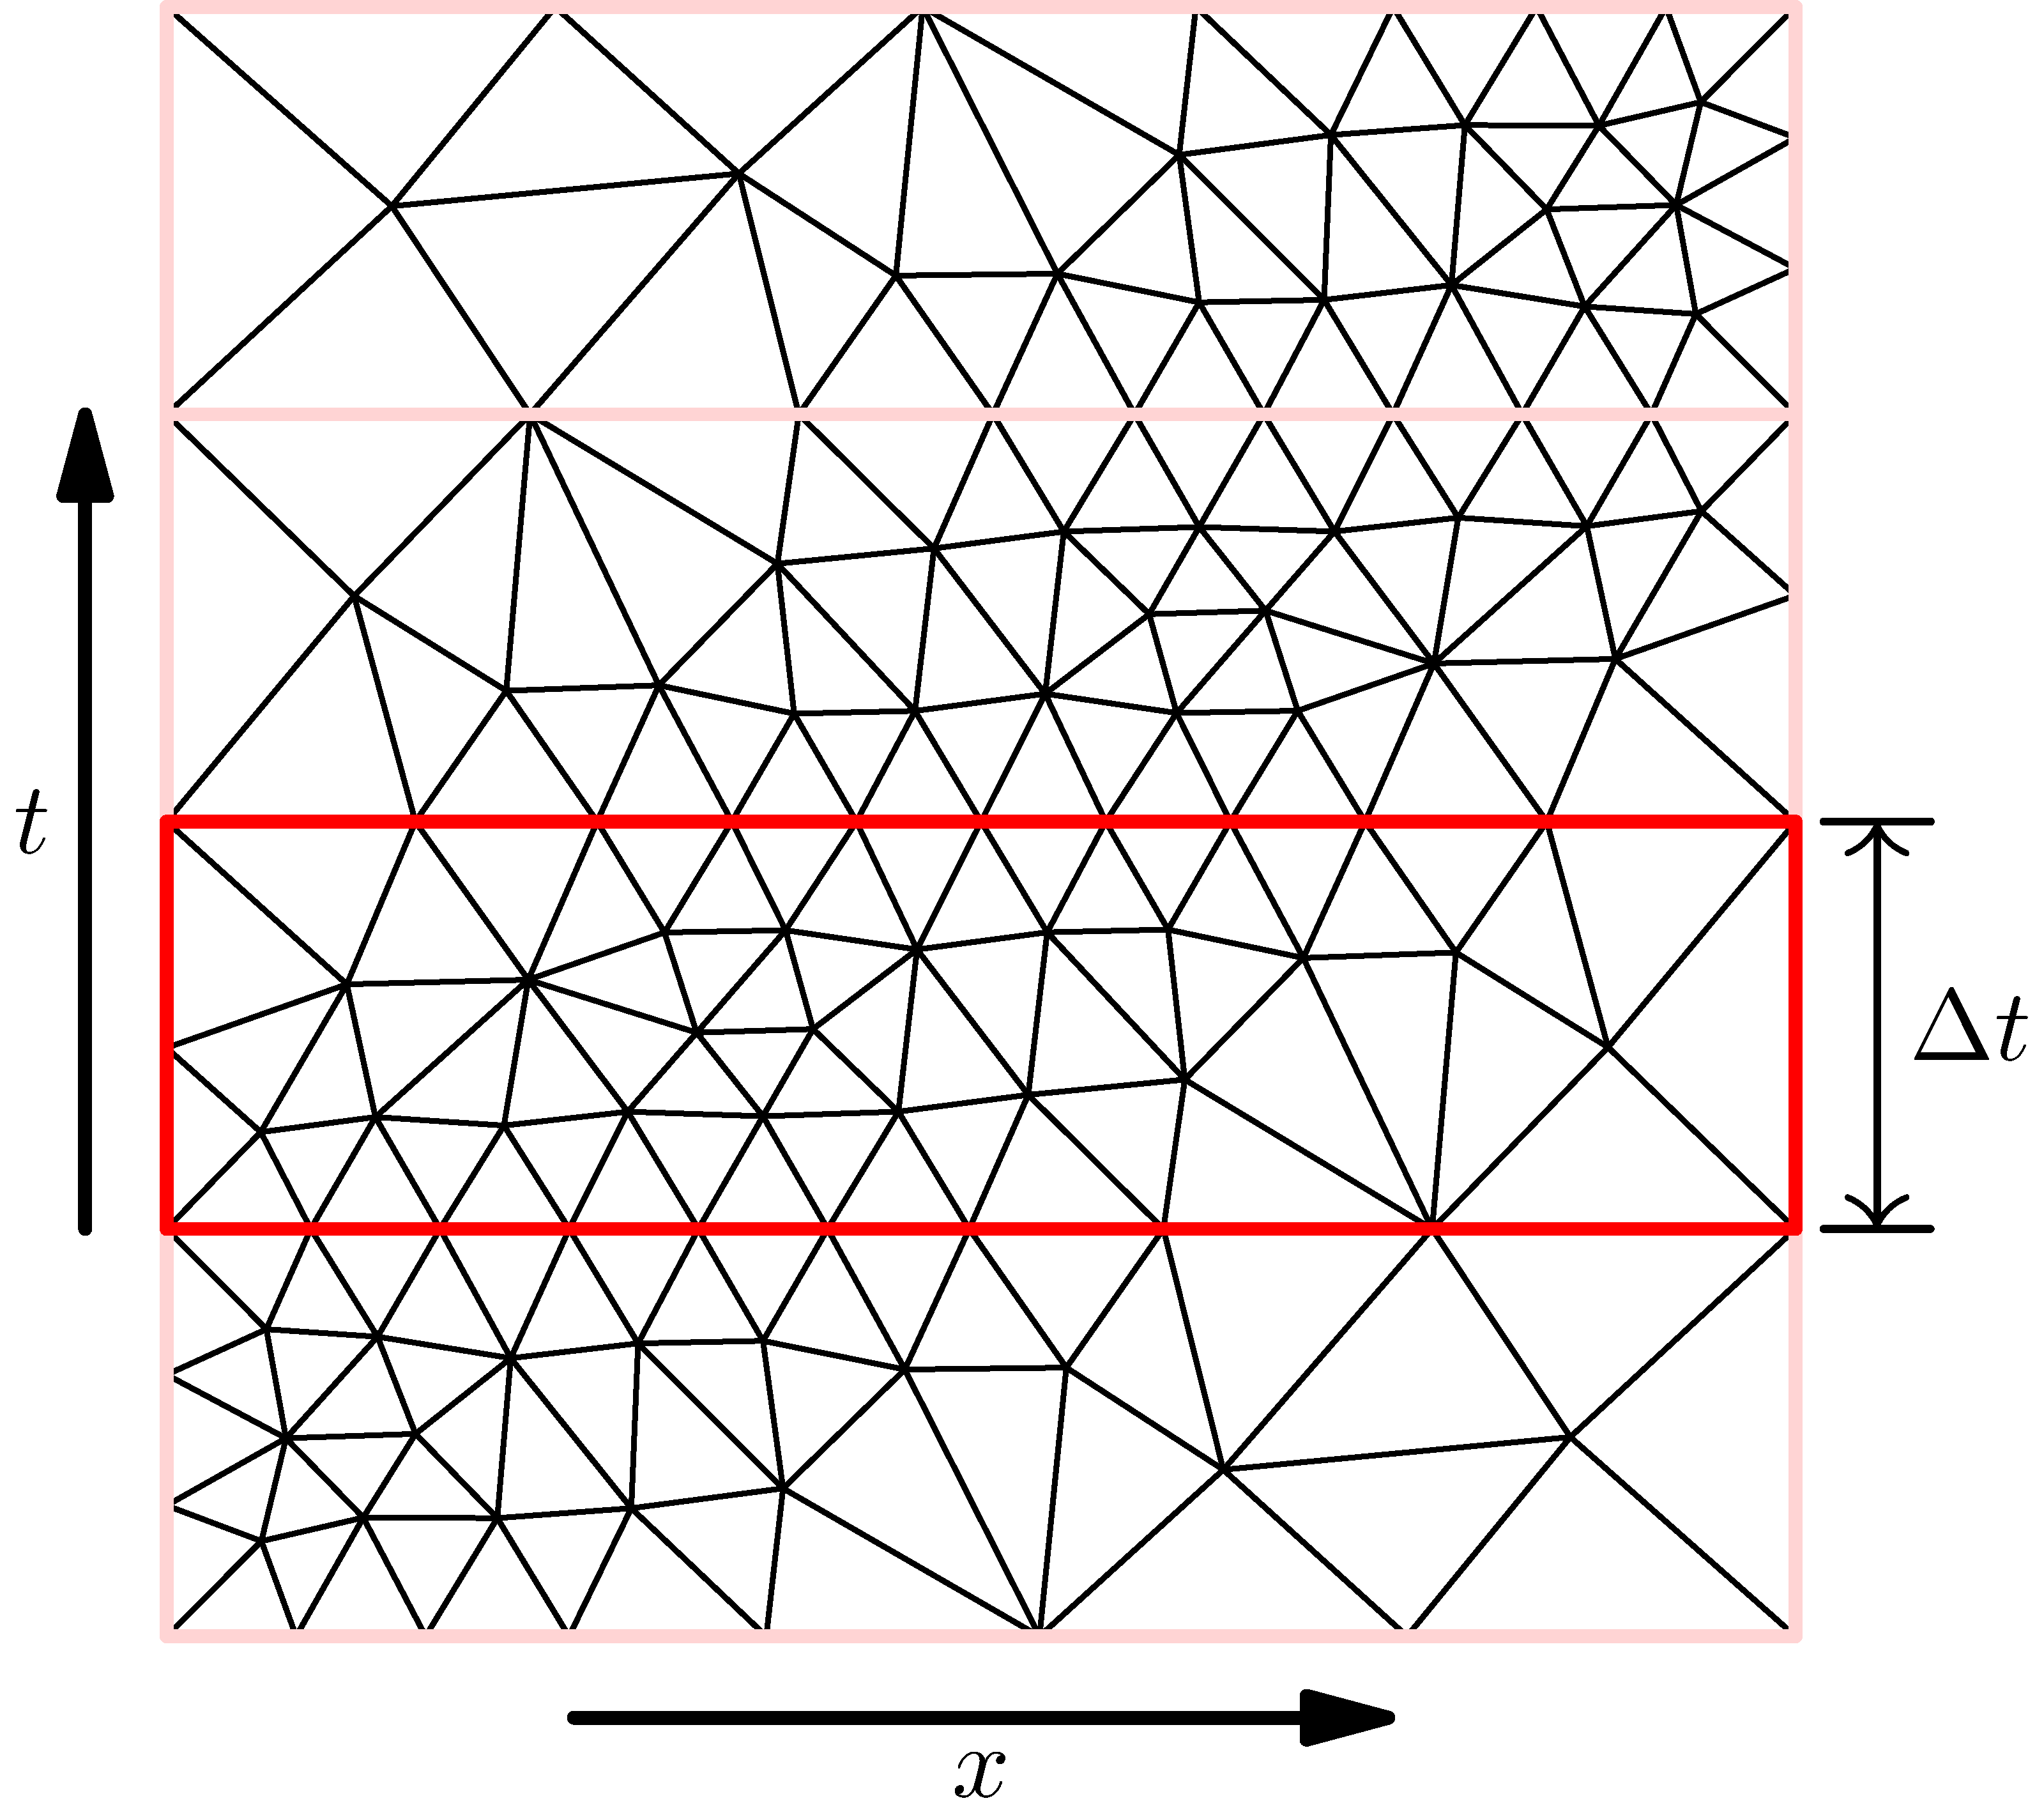
\includegraphics[width=0.6\textwidth]{figures/wave_2D.png}
    \caption{时空混合离散间断伽辽金法网格划分}
    \label{fg:slab}
\end{figure}

针对波动方程分析中的数值色散问题,最直接的解决方案是控制时间域和空间域节点间距满足稳定性条件要求\cite{bajer1986}。
江小燕和王建国\cite{JiangXiaoYan2014}针对动力问题的时间有限元法采用谱半径方法进行稳定性分析,以此确定稳定的时域节点间距。
然而,对于分均布节点分布下的高维问题,无论是稳定性分析还是控制节点间距都将是巨大的挑战。
在求解过程中添加以微分方程为基础的稳定项也可以在一定程度上缓解数值色散问题,如迎风型彼得罗夫伽辽金法(SUPG)\cite{hughes1988}、最小二乘伽辽金法(GLS)\cite{hughes2000}、变分多尺度模型(VMS)\cite{hughes1996}等。
该类方法中强形式需要形函数的高阶导数参与计算,并且可能引入数值耗散问题影响计算精度。
相较于前两类方法,采用时域高阶近似适用于任意节点分布情况,更适合用于抑制时空混合离散分析中的数值色散问题。
Petersen等人\cite{petersen2000}根据波动方程的通解,引入波速相关的高阶完备多项式近似方案。
Banjai等人\cite{banjai2017}采用用Trefftz多项式近似方法,该近似方法在传统波动问题及Helmholtz问题中具有较高的计算精度。
Wriggers和Junker\cite{wriggers2024}则是在虚单位近似的框架下直接引入高阶多项式作为基函数。
\textbf{上述高阶近似方法基函数在全域上并不连续,需要引入单元间位移约束保证空间方向上的连续性。并且缺乏时空混合离散下数值色散问题稳定性分析理论,以确定稳定状态下的近似基函数阶次和表达式。}

无网格法通常指不需要依赖网格拓扑信息建立形函数的分析方法,如光滑水动力学法\cite{Yang2019,Chang2011}、物质点法\cite{Kan2022}、无单元伽辽金法\cite{Wu2016d,Cheng2024}、径向基函数法\cite{jiang2025}、物理信息依赖核函数配点法\cite{FuZhuoJia2022}、近场动力学\cite{Gu2016,Zhang2022}、再生核配点法\cite{Hu2023}等。
在时空混合离散无网格法方面,Myers等人\cite{myers2002}首次提出时空混合离散径向基函数,并结合配点法进行求解。
林继等人\cite{lin2021}将径向基函数和三角函数引入配点型反向迭代法中求解对流扩散问题。
Huang等人\cite{huang2023}采用时空混合离散的边界移动最小二乘近似结合配点法求解弹性问题。
上述时空混合离散无网格法中均基于强形式型的配点法建立,而不是采用基于哈密顿原理的伽辽金弱形式进行求解。
原因主要是伽辽金法中涉及数值积分,而无网格形函数通常为有理式,无法进行准确数值积分,难以保证误差收敛率\cite{wu2021}。
为保证求解精度,伽辽金无网格法需要采用变分一致的数值积分方案\cite{Wu2016d}。
申请人针对变分一致型伽辽金无网格数值积分方案提出了嵌套子域积分法\cite{wang2016b}和再生光滑梯度积分法\cite{wang2019a}。
其中的\textbf{再生光滑梯度积分法理论框架适用于任意维度和任意阶次基函数的无网格近似,可推广至高维时空混合离散问题,缓解数值色散现象,提高时空混合离散伽辽金无网格法计算精度。}

综上所述,
时空混合离散伽辽金法可保持全域系统能量守恒,适用于自适应节点加密及大规模并行计算过程。
但是,该方法仍然存在诸多基础理论和难点问题导致其无法适用于任意节点分布情况,包括:时域末端本质边界条件施加问题、数值色散问题和高维度网格划分问题。
无网格法则具有全域连续高阶光滑形函数,可用于缓解波动问题分析中的数值色散问题。
依据节点信息建立形函数的特点,无网格法适用于时空混合离散自适应节点加密过程。
近年,申请人及其合作者针对伽辽金无网格法开展了系列研究工作,如变分一致性伽辽金无网格法本质边界条件施加方法\cite{Wu2022b,wu2023,wu2024}、伽辽金无网格法精度分析\cite{wu2021,wu2018a}、伽辽金无网格法数值积分方案\cite{Wu2016d,wang2016b,wang2019a}等。
本项目拟在此基础上提出时空混合离散伽辽金法中虚位移本质边界条件施加方案;
对时空混合离散伽辽金法进行稳定性分析,建立可缓解数值色散问题的再生核近似方案;
并引入再生光滑梯度积分理论框架,降低高维背景积分域划分难度。
以此,建立适用于任意节点分布的伽辽金无网格分析方法。
项目研究成果将有助于时空混合离散分析理论的深入发展,推动该方法在科学研究和工程领域上的应用。

\vspace{-5pt}

\begin{REF}
	\subsection*{参考文献}
	\vspace{-50pt}
	\bibliographystyle{gbt7714-2005-numerical}
	\bibliography{ref}%参考文献
\end{REF}

\newpage%自己判断是否需要
